\newpage
\subsubsection{Dynamic Model}
This is the dynamic model for the system. When the user accesses the frontend, they can either request to 
publish or verify a document on the blockchain. The backend updates and publishes the document to 
the blockchain or verifies the requested document. The backend then returns the information about the supplied 
document (audit trail, past versions) or about the updated 
blockchain (location, owner) to the user. 

\begin{figure}[h]
\centering % centre is you want
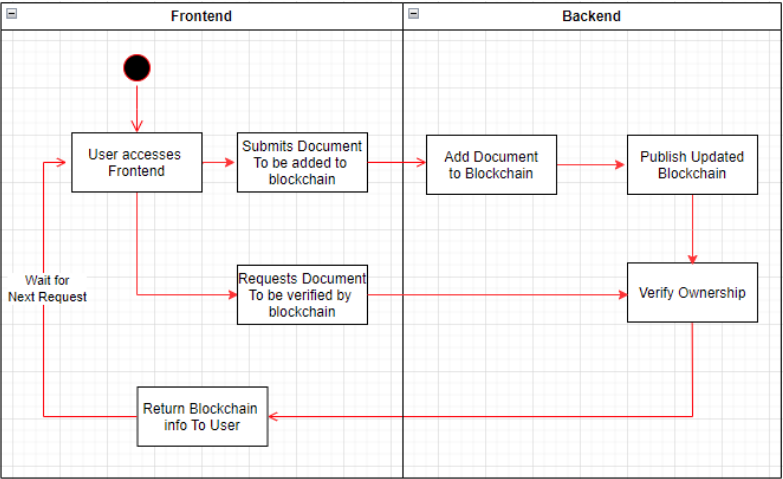
\includegraphics[scale=0.50]{dynamic-model} 
\caption{Dynamic model of the system}
\label{fig: dynamic-model} % Can be used with function \ref{fig: passion-fruit-flower} to reference to image
\end{figure}
\newpage
